\documentclass[12pt,a4paper]{article}

% Данные для титульной страницы

% Номер лабораторной работы
\newcommand{\labnumber}{9}

% Название работы
\newcommand{\labtitle}{Строки в языке СИ}

% Группа студента
\newcommand{\group}{ПО-4}

% Студент, выполнивший работу
\newcommand{\labauthor}{Галанин П. И.}

% Должность преподавателя
\newcommand{\teacherstatus}{ст. преподаватель}

% Преподаватель
\newcommand{\teacher}{Хацкевич М. В.}

% Дата
\newcommand{\labdate}{2020}

% Подключение стилевого файла
\usepackage{../labwork} 

% Используемые языки программирования в исходниках в отчете
\lstloadlanguages{C}



\begin{document}



% Добавляем титульный лист
\maketitle



% Заголовок
\labheading



% Цель работы
\begin{labgoal}
Изученить принципы обработки строк в языке Си: ввод-вывод строк, использование стандартных функций языка С, работа с памятью.
\end{labgoal}



% Метка начала отчета по работе
\labreport

\section{Task A14}

\begin{conductionA14}
Условие: Дана строка, содержащая полное имя файла, то есть имя диска, список
каталогов (путь), собственно имя и расширение. Выделить из этой строки имя
файла, а по расширению определить, что это за файл (например: «exe» -
исполняемый, «gif», «jpg» - графический, «doc» - текстовый документ и т.д.).
\end{conductionA14}

Исходный код программы изображен на листинге \ref{lst:lab9-a14}.

Вывод программы при jpg-файле на рисунке \ref{fig:a14-jpg}.

Вывод программы при doc-файле на рисунке \ref{fig:a14-doc}.

Вывод программы при exe-файле на рисунке \ref{fig:a14-exe}.

Вывод программы при exe-файле на рисунке \ref{fig:a14-gif}.

Вывод программы при exe-файле на рисунке \ref{fig:a14-none}.

\lstinputlisting[
  language=C,
  caption={Task A 14},
  label={lst:lab9-a14}
]{a14.c}

% Вставляем изображение
\begin{figure}[ht]
  \centering
  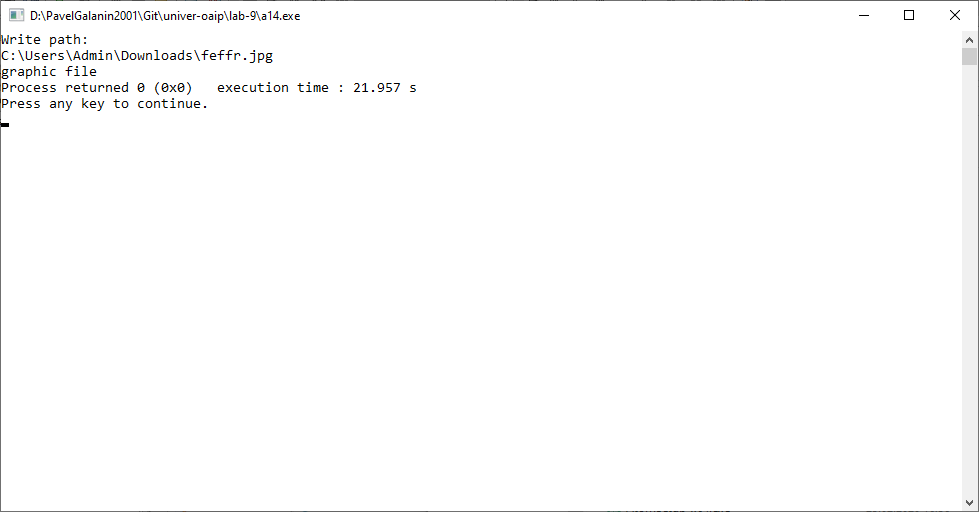
\includegraphics[width=16cm]{imgs/a14jpg.png}
  \caption{Task A 14: jpg file}
  \label{fig:a14-jpg}
\end{figure}

% Вставляем изображение
\begin{figure}[ht]
  \centering
  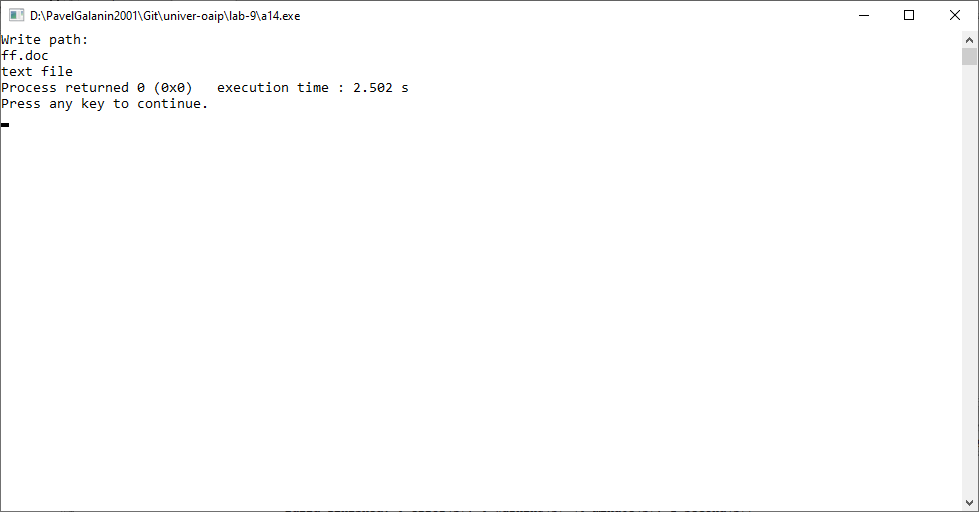
\includegraphics[width=16cm]{imgs/a14doc.png}
  \caption{Task A 14: doc file}
  \label{fig:a14-doc}
\end{figure}

% Вставляем изображение
\begin{figure}[ht]
  \centering
  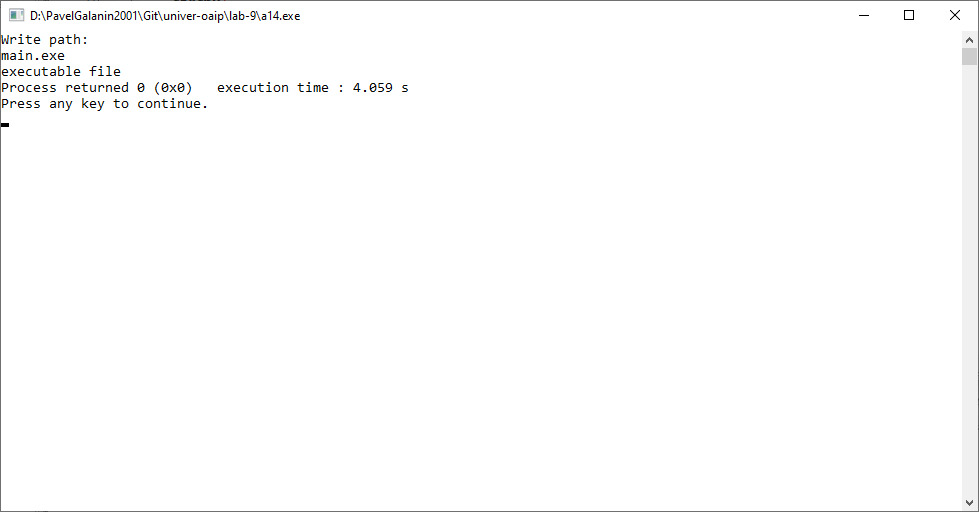
\includegraphics[width=16cm]{imgs/a14exe.png}
  \caption{Task A 14: exe file}
  \label{fig:a14-exe}
\end{figure}

% Вставляем изображение
\begin{figure}[ht]
  \centering
  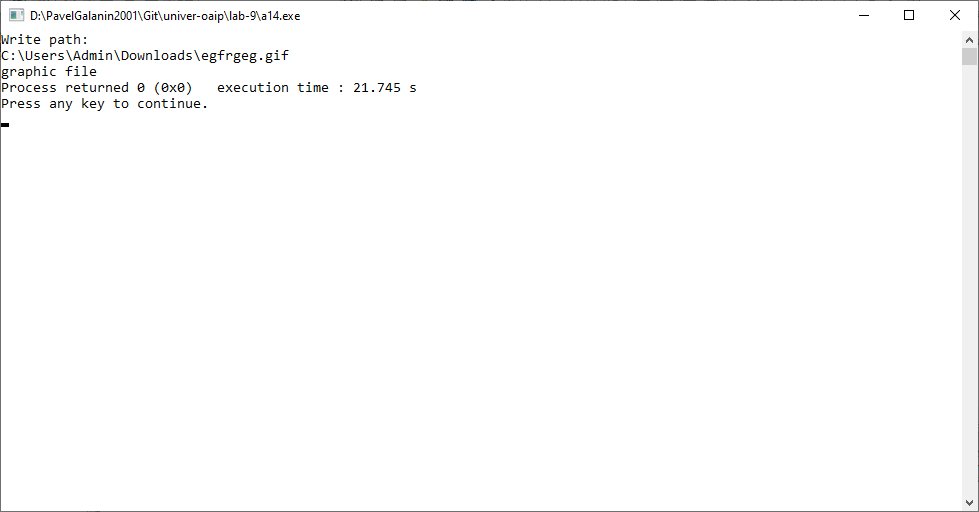
\includegraphics[width=16cm]{imgs/a14gif.png}
  \caption{Task A 14: gif file}
  \label{fig:a14-gif}
\end{figure}

% Вставляем изображение
\begin{figure}[ht]
  \centering
  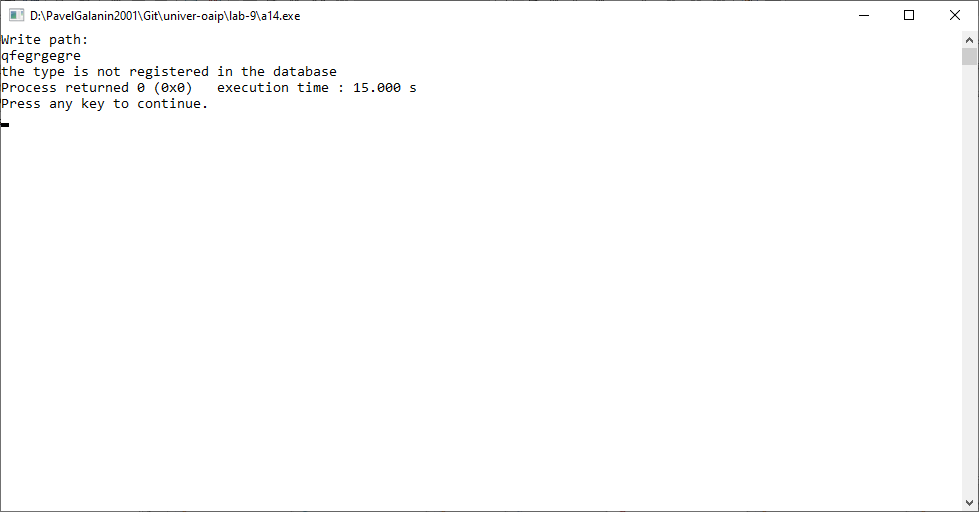
\includegraphics[width=16cm]{imgs/a14none.png}
  \caption{Task A 14: don't known type}
  \label{fig:a14-none}
\end{figure}

\clearpage

\section{Task B12}

\begin{conductionB12}
Условие: Ввести строку, содержащую несколько слов. Выбрать те слова, в
которых первая буква этого слова встречается еще хоть один раз.
\end{conductionB12}

Исходный код программы изображен на листинге \ref{lst:lab9-b12}.

Вывод программы на рисунке\ref{fig:a14-none}.

Вывод программы на рисунке\ref{fig:a14-none}.

\lstinputlisting[
  language=C,
  caption={Task B 12},
  label={lst:lab9-b12}
]{b12.c}

% Вставляем изображение
\begin{figure}[ht]
  \centering
  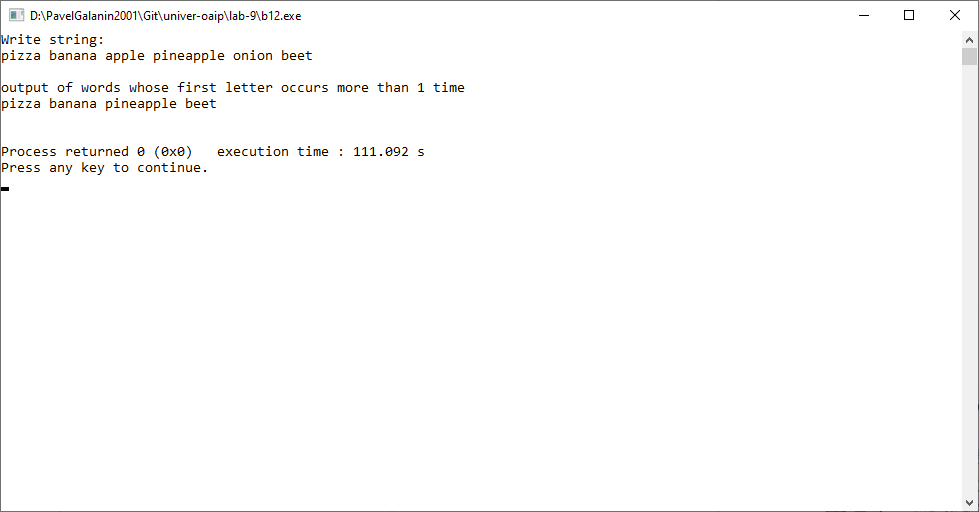
\includegraphics[width=16cm]{imgs/b12-test1.png}
  \caption{Task B 12: test1}
  \label{fig:b12-test1}
\end{figure}

% Вставляем изображение
\begin{figure}[ht]
  \centering
  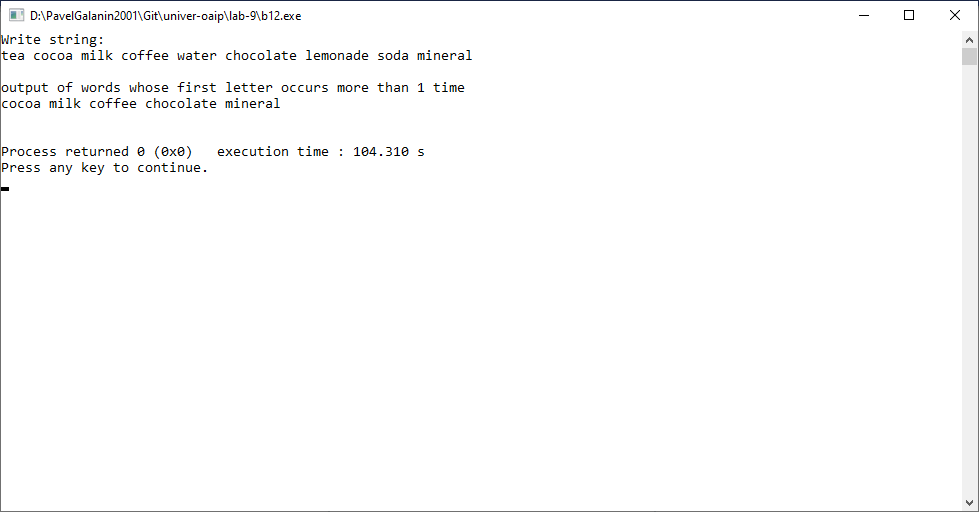
\includegraphics[width=16cm]{imgs/b12-test2.png}
  \caption{Task B 12: test2}
  \label{fig:b12-test2}
\end{figure}



\clearpage

\section{Вывод}

Попробовали на практике со строками в Си:

Поработали над строками с библиотекой string.h:

\begin{itemize}
    \item strtok() - разделяли строку на лексемы
    \item strlen() - узнавали размер строки
    \item strcpy() - копировали строку в строку
\end{itemize}

Поработали над строками с библиотекой stdio.h:

\begin{itemize}
    \item gets() - ввод строки
    \item printf() - вывод строки
\end{itemize}

Поработали с динамической памятью с библиотекой stdlib.h:

\begin{itemize}
    \item calloc() - создавали динамические массивы
    \item free() - освобождали память
\end{itemize}

\end{document}
